\clearpage
\section{Voice flow}
\label{sec:voice_flow}
\subsection{Attori dei casi d'uso}
\label{sec:attori_uc}
\subsubsection{Attori primari}
%immagine gerarchio utilizzo + didascalia
\begin{itemize}
	\item  Utente generico: Utente che, indipendentemente dal fatto che abbia effettuato il login o meno, accede all'applicazione.
	\item  Utente non autenticato: Utente che non ha effettuato il login.
	\item  Utente autenticato: Utente che ha completato la procedura di autenticazione.
\end{itemize}
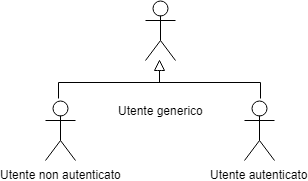
\includegraphics[width=1\textwidth]{../includes/pics/primari.png}
\subsection{Elenco dei casi d'uso}
\label{sec:elenco_uc}
%immagine attori che accedono a casi d'uso+didascalia
\subsubsection{UC1 - Presentazione funzionalità}
\begin{itemize}
	\item  Attori primari:  Utente generico
	\item  Scopo e descrizione: viene presentato all'utente una breve guida illustrata che permette di capire cosa è possibile fare con l'applicazione.
	\item  Scenario principale: l'utente legge la presentazione.
	\item  Pre-condizione: il sistema è funzionante e raggiungibile.
	\item  Post-condizione: l'utente è stato informato di alcune abilità del sistema.
\end{itemize}